% Documentclass til dobbeltsidet udskrift på papir.
\documentclass[english,a4paper,11pt,fleqn,dvipsnames,oneside,openright]{memoir} 	
% Openright aabner kapitler paa hoejresider (openany begge)
% Documentclass til PDF format
%\documentclass[danish,a4paper,11pt,fleqn,dvipsnames,oneside]{memoir} 	

% Kommentarer og rettelser med \fxnote. Med 'final' i stedet for 'draft' udloeser hver note en error i den faerdige rapport.
\usepackage[footnote,draft,english,silent,nomargin]{fixme}
%\usepackage[final,footnote,english,silent,nomargin]{fixme}

%%%% PACKAGES %%%%
\newcommand{\shellcmd}[1]{\texttt{\footnotesize\# #1}\\}
%%%% P OF THE BOX %%%%
\usepackage{pbox}

% ¤¤ Oversaettelse og tegnsaetning ¤¤ %
\usepackage[utf8]{inputenc}					% Input-indkodning af tegnsaet (UTF8)
\usepackage[english]{babel}					% Dokumentets sprog
\usepackage[T1]{fontenc}					% Output-indkodning af tegnsaet (T1)
\usepackage{ragged2e,anyfontsize}			% Justering af elementer
% ¤¤ Figurer og tabeller (floats) ¤¤ %
\usepackage{array}
\usepackage{booktabs}
\newcolumntype{L}[1]{>{\raggedright\let\newline\\\arraybackslash\hspace{0pt}}m{#1}}
\newcolumntype{C}[1]{>{\centering\let\newline\\\arraybackslash\hspace{0pt}}m{#1}}
\newcolumntype{R}[1]{>{\raggedleft\let\newline\\\arraybackslash\hspace{0pt}}m{#1}}

\newcommand{\otoprule}{\midrule[\heavyrulewidth]}

\usepackage{longtable}
\usepackage{graphicx} 						% Haandtering af eksterne billeder (JPG, PNG, EPS, PDF)
%\usepackage{eso-pic}						% Tilfoej billedekommandoer paa hver side
%\usepackage{wrapfig}						% Indsaettelse af figurer omsvoebt af tekst. \begin{wrapfigure}{Placering}{Stoerrelse}
\usepackage{multirow}                		% Fletning af raekker og kolonner (\multicolumn og \multirow)
\usepackage{multicol}         	        	% Muliggoer output i spalter
\usepackage{rotating}						% Rotation af tekst med \begin{sideways}...\end{sideways}
\usepackage{colortbl} 						% Farver i tabeller (fx \columncolor og \rowcolor)
\usepackage[x11names]{xcolor}         				% Definer farver med \definecolor. Se mere: http://en.wikibooks.org/wiki/LaTeX/Colors
\usepackage{flafter}						% Soerger for at floats ikke optraeder i teksten foer deres reference
\let\newfloat\relax 						% Justering mellem float-pakken og memoir
\usepackage{float}							% Muliggoer eksakt placering af floats, f.eks. \begin{figure}[H]

\usepackage[section]{placeins}

% ¤¤ Matematik mm. ¤¤
\usepackage{amsmath,amssymb,stmaryrd} 		% Avancerede matematik-udvidelser
\usepackage{mathtools}						% Andre matematik- og tegnudvidelser
\usepackage{textcomp}                 		% Symbol-udvidelser (f.eks. promille-tegn med \textperthousand )
\usepackage{rsphrase}						% Kemi-pakke til RS-saetninger, f.eks. \rsphrase{R1}
\usepackage[version=3]{mhchem} 				% Kemi-pakke til flot og let notation af formler, f.eks. \ce{Fe2O3}
\usepackage{siunitx}						% Flot og konsistent praesentation af tal og enheder med \si{enhed} og \SI{tal}{enhed}
\sisetup{output-decimal-marker = {,}}		% Opsaetning af \SI (DE for komma som decimalseparator) 

% ¤¤ Referencer og kilder ¤¤ %
\usepackage[danish]{varioref}				% Muliggoer bl.a. krydshenvisninger med sidetal (\vref)
%\usepackage[numbers]{natbib}							% Udvidelse med naturvidenskabelige citationsmodeller
\usepackage{xr}							    % Referencer til eksternt dokument med \externaldocument{<NAVN>}
%\usepackage{glossaries}					% Terminologi- eller symbolliste (se mere i Daleifs Latex-bog)

% ¤¤ Misc. ¤¤ %
%\usepackage[bottom]{footmisc}
\usepackage{enumerate}
\usepackage{easylist}                       % enumerate og itemize
\usepackage{listings}						% Placer kildekode i dokumentet med \begin{lstlisting}...\end{lstlisting}
\usepackage{lipsum}							% Dummy text \lipsum[..]
\usepackage[shortlabels]{enumitem}			% Muliggoer enkelt konfiguration af lister
\usepackage{pdfpages}						% Goer det muligt at inkludere pdf-dokumenter med kommandoen \includepdf[pages={x-y}]{fil.pdf}	
\pdfoptionpdfminorversion=6					% Muliggoer inkludering af pdf dokumenter, af version 1.6 og hoejere
\pretolerance=2500 							% Justering af afstand mellem ord (hoejt tal, mindre orddeling og mere luft mellem ord)

%%%% CUSTOM SETTINGS %%%%

% ¤¤ Marginer ¤¤ %
\setlrmarginsandblock{3.5cm}{2.5cm}{*}		% \setlrmarginsandblock{Indbinding}{Kant}{Ratio}
\setulmarginsandblock{2.5cm}{3.0cm}{*}		% \setulmarginsandblock{Top}{Bund}{Ratio}
\checkandfixthelayout 						% Oversaetter vaerdier til brug for andre pakker

%	¤¤ Afsnitsformatering ¤¤ %
\setlength{\parindent}{0mm}           		% Stoerrelse af indryk
\setlength{\parskip}{3mm}          			% Afstand mellem afsnit ved brug af double Enter
\linespread{1,1}							% Linie afstand

% ¤¤ Litteraturlisten ¤¤ %
%\bibpunct[,]{[}{]}{;}{a}{,}{,} 				% Definerer de 6 parametre ved Harvard henvisning (bl.a. parantestype og seperatortegn)
\bibliographystyle{unsrtnat}			% Udseende af litteraturlisten.
\usepackage[backend=biber, sorting=none, style=numeric]{biblatex}
\bibliography{../bibliography.bib}


% ¤¤ Indholdsfortegnelse ¤¤ %
\setsecnumdepth{subsection}		 			% Dybden af nummerede overkrifter (part/chapter/section/subsection)
\maxsecnumdepth{subsection}					% Dokumentklassens graense for nummereringsdybde
\settocdepth{subsection} 					% Dybden af indholdsfortegnelsen

% ¤¤ Lister ¤¤ %
\setlist{
  topsep=0pt,								% Vertikal afstand mellem tekst og listen
  itemsep=-1ex,								% Vertikal afstand mellem items
} 

% ¤¤ Visuelle referencer ¤¤ %
\usepackage[colorlinks]{hyperref}			% Danner klikbare referencer (hyperlinks) i dokumentet.
\hypersetup{colorlinks = true,				% Opsaetning af farvede hyperlinks (interne links, citeringer og URL)
    linkcolor = black,
    citecolor = black,
    urlcolor = black
}

% ¤¤ Opsaetning af figur- og tabeltekst ¤¤ %
\captionnamefont{\small\bfseries\itshape}	% Opsaetning af tekstdelen ('Figur' eller 'Tabel')
\captiontitlefont{\small}					% Opsaetning af nummerering
\captiondelim{. }							% Seperator mellem nummerering og figurtekst
\hangcaption								% Venstrejusterer flere-liniers figurtekst under hinanden
\captionwidth{\linewidth}					% Bredden af figurteksten
\setlength{\belowcaptionskip}{0pt}			% Afstand under figurteksten
		
% ¤¤ Opsaetning af listings ¤¤ %

\definecolor{commentGreen}{RGB}{34,139,24}
\definecolor{stringPurple}{RGB}{208,76,239}

\lstset{language=Matlab,					% Sprog
	basicstyle=\ttfamily\scriptsize,		% Opsaetning af teksten
	keywords={for,if,while,else,elseif,		% Noegleord at fremhaeve
			  end,break,return,case,
			  switch,function},
	keywordstyle=\color{blue},				% Opsaetning af noegleord
	commentstyle=\color{commentGreen},		% Opsaetning af kommentarer
	stringstyle=\color{stringPurple},		% Opsaetning af strenge
	showstringspaces=false,					% Mellemrum i strenge enten vist eller blanke
	numbers=left, numberstyle=\tiny,		% Linjenumre
	extendedchars=true, 					% Tillader specielle karakterer
	columns=flexible,						% Kolonnejustering
	breaklines, breakatwhitespace=true,		% Bryd lange linjer
}

% ¤¤ Navngivning ¤¤ %
\addto\captionsdanish{
	\renewcommand\appendixname{Appendiks}
	\renewcommand\contentsname{Indholdsfortegnelse}	
	\renewcommand\appendixpagename{Appendiks}
	\renewcommand\appendixtocname{Appendiks}
	\renewcommand\cftchaptername{\chaptername~}				% Skriver "Kapitel" foran kapitlerne i indholdsfortegnelsen
	\renewcommand\cftappendixname{\appendixname~}			% Skriver "Appendiks" foran appendiks i indholdsfortegnelsen
}

% ¤¤ Kapiteludssende ¤¤ %
\definecolor{numbercolor}{gray}{0.7}		% Definerer en farve til brug til kapiteludseende
\newif\ifchapternonum

\makechapterstyle{jenor}{					% Definerer kapiteludseende frem til ...
  \renewcommand\beforechapskip{0pt}
  \renewcommand\printchaptername{}
  \renewcommand\printchapternum{}
  \renewcommand\printchapternonum{\chapternonumtrue}
  \renewcommand\chaptitlefont{\fontfamily{pbk}\fontseries{m}\fontshape{n}\fontsize{25}{35}\selectfont\raggedleft}
  \renewcommand\chapnumfont{\fontfamily{pbk}\fontseries{m}\fontshape{n}\fontsize{1in}{0in}\selectfont\color{numbercolor}}
  \renewcommand\printchaptertitle[1]{%
    \noindent
    \ifchapternonum
    \begin{tabularx}{\textwidth}{X}
    {\let\\\newline\chaptitlefont ##1\par} 
    \end{tabularx}
    \par\vskip-2.5mm\hrule
    \else
    \begin{tabularx}{\textwidth}{Xl}
    {\parbox[b]{\linewidth}{\chaptitlefont ##1}} & \raisebox{-15pt}{\chapnumfont \thechapter}
    \end{tabularx}
    \par\vskip2mm\hrule
    \fi
  }
}											% ... herz


\chapterstyle{jenor}						% Valg af kapiteludseende - Google 'memoir chapter styles' for alternativer

% ¤¤ Sidehoved ¤¤ %

\makepagestyle{AU}							% Definerer sidehoved og sidefod udseende frem til ...
\makepsmarks{AU}{%

	\createplainmark{lof}{both}{\listfigurename}
	\createplainmark{lot}{both}{\listtablename}
	\createplainmark{bib}{both}{\bibname}
	\createplainmark{index}{both}{\indexname}
	\createplainmark{glossary}{both}{\glossaryname}
}
\nouppercaseheads											% Ingen Caps oenskes

\makeevenhead{AU}{Group INTRO-760}{}{\leftmark}				    % Definerer lige siders sidehoved (\makeevenhead{Navn}{Venstre}{Center}{Hoejre})
\makeoddhead{AU}{\rightmark}{}{Aalborg University - Energy Technology}		% Definerer ulige siders sidehoved (\makeoddhead{Navn}{Venstre}{Center}{Hoejre})
\makeevenfoot{AU}{\thepage}{}{}							    % Definerer lige siders sidefod (\makeevenfoot{Navn}{Venstre}{Center}{Hoejre})
\makeoddfoot{AU}{}{}{\thepage/\thelastpage}								% Definerer ulige siders sidefod (\makeoddfoot{Navn}{Venstre}{Center}{Hoejre})
\makeheadrule{AU}{\textwidth}{0.5pt}						% Tilfoejer en streg under sidehovedets indhold
\makefootrule{AU}{\textwidth}{0.5pt}{1mm}					% Tilfoejer en streg under sidefodens indhold

\copypagestyle{AUchap}{AU}								    % Sidehoved for kapitelsider defineres som standardsider, men med blank sidehoved
\makeoddhead{AUchap}{}{}{}
\makeevenhead{AUchap}{}{}{}
\makeheadrule{AUchap}{\textwidth}{0pt}
\aliaspagestyle{chapter}{AUchap}							% Den ny style vaelges til at gaelde for chapters
															% ... her
															
\pagestyle{AU}												% Valg af sidehoved og sidefod


%%%% CUSTOM COMMANDS %%%%

% ¤¤ Billede hack ¤¤ %
\newcommand{\figur}[4]{
		\begin{figure}[htbp] \centering
			\includegraphics[width=#1\textwidth]{Images/#2}
			\caption{#3}\label{fig:#4}
		\end{figure} 
}

% ¤¤ Specielle tegn ¤¤ %
\newcommand{\decC}{^{\circ}\text{C}}
\newcommand{\dec}{^{\circ}}
\newcommand{\m}{\cdot}


%%%% ORDDELING %%%%

\hyphenation{}

%%% kloge referencer %%%% skal være sidst
\usepackage{cleveref}

\newcommand{\quotemark}[1]{``#1''} % Quote with the command \quotemark{text}

%%\usepackage[backend=biber]{biblatex}    
\usepackage[style=english]{csquotes}
\usepackage{pdflscape}
\usepackage[export]{adjustbox}

\newcommand\tab[1][1cm]{\hspace*{#1}}

\begin{document}
	
\begin{titlingpage}

	
\newcommand{\HRule}{\rule{\linewidth}{0.1mm}} % Defines a new command for the horizontal lines, change thickness here

\vspace*{-2cm}
\begin{figure}[htbp]
	\begin{center}
		
\includegraphics[width=\textwidth]{../Pictures/AAU_logo}
		\label{aau_logo}
	\end{center}	
\end{figure}

\vspace*{2cm}
\begin{figure}[htbp]
	\begin{center}
		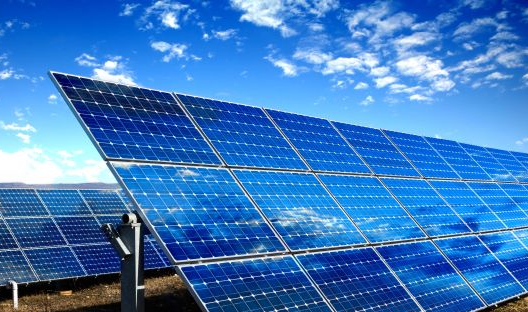
\includegraphics[width=\textwidth]{../Pictures/frontpage_pvpanel.png}
		\label{frontpage}
	\end{center}	
\end{figure}

\begin{center}
\vspace*{0.5cm}
\HRule \\[0.8cm]
{\huge \bfseries \textsc{DC-DC Converter for PV Module Integration}}\\[0.2cm]
\HRule \\[1.5cm]

\textsc{\textbf{Estefanía Ruiz, Aitor Teran, Nicolai H. Fransen, Jesper Kloster, Thassilo Lang \& Nicolás Murguizur Bustos}}


\vspace*{1cm}
\textsc{\textbf{Supervisors: Lajos Török \& Dezso Sera}}
\end{center}
\end{titlingpage}

\vspace*{1cm}
\begin{table}[H]
	\begin{tabular}{l l} 
		\textbf{Title} &  \textbf{DC-DC Converter for PV Module Integration} \\ 
		\textbf{Semester} & \textbf{$7^{th}$ INTRO}  \\ 
		\textbf{Project Period} & \textbf{10.09.2018 - 19.12.2018}  \\ 
		\textbf{ECTS} &  \textbf{10}\\ 
		\textbf{Supervisors} & \textbf{Lajos Török \& Dezso Sera}  \\ 
		\textbf{Group} & \textbf{INTRO-760}  \\ 
	\end{tabular}
\end{table}

%\vspace*{1cm}
\begin{center}	
	\vspace{40pt}
	\begin{minipage}{0.4\linewidth}
		\centering
		\hrule
		\vspace{12pt}
		Estefanía Ruiz\\ 
		20181097
	\end{minipage}
	\hspace{10pt}
	\vspace{40pt}
	\begin{minipage}{0.4\linewidth}
		\centering
		\hrule
		\vspace{12pt}
		Aitor Teran\\ 
		20186474	
	\end{minipage}
	\hspace{10pt}
	\vspace{40pt}
	\begin{minipage}{0.4\linewidth}
		\centering
		\hrule
		\vspace{12pt}
		Nicolai H. Fransen\\
		20181094
	\end{minipage}
	\hspace{10pt}
	\begin{minipage}{0.4\linewidth}
		\centering
		\hrule
		\vspace{12pt}
		Jesper Kloster\\
		20181081 
	\end{minipage}
	\hspace{10pt}
	\begin{minipage}{0.4\linewidth}
		\centering
		\hrule
		\vspace{12pt}
		Thassilo Lang\\ 
		20186559 
	\end{minipage}
	\hspace{10pt}
	\vspace{20pt}
	\begin{minipage}{0.4\linewidth}
		\centering
		\hrule
		\vspace{12pt}
		Nicolás Murguizur Bustos\\ 
		20181086
	\end{minipage}
\end{center}

%\vspace{3cm}
\begin{tcolorbox}
\textbf{Synopsis:}\newline
PV modules must work at their maximum power point in order to achieve the highest overall efficiency. Several environmental conditions can affect the output power of the PV modules.\newline
This project will address these problems, by implementing a MIC including a MPPT algorithm. The MIC will minimize the power losses and therefore increase the efficiency.\newline
The purpose of this report is to define the boundaries of the project. This includes the main objectives and the initial research. Furthermore there have been included a gantt chart of the entire project.
\end{tcolorbox}

\vspace*{0.5cm}
\textbf{By signing the document, members of the group accepts that the entire group have participated in the work of the report. Therefore, all members vouch for the content of the report, and confirms that it doesn't include plagiarism.}

\clearpage
\tableofcontents

\chapter*{Preface}

This paper describes the "P0" report of the group project "DC-DC converter for PV module integration." It has been developed from the 10. of September to the 9. of October 2018, at Aalborg University, Institut of Energy by the group INTRO-760.

The "P0" is an initially report which discusses research about maximizing the power from PV modules.
Furthermore a theoretically comparison between different converter topologies has been done. After "P0" there will be a "P1" report which will include the entire project.

The literature references are shown in square brackets, with a number referring to a specific document which can be found in the bibliography. Pictures and tables will be denoted in the X,Y format, with X representing the chapter and Y the figure or table number. 

The process and development of "P0" has been based on the Problem Based Learning $(PBL)$ method. The group will continue using this method for the "P1" report           
\chapter*{Summary}
\input{docs/Nomenclature.tex}

\chapter{Introduction}




To this date, sustainable energy sources have become an area in focus worldwide in an attempt to reduce the environmental impact due to emissions of CO2 and other greenhouse gasses. The development of competitive systems to exploit renewable energy sources is the best alternative to reduce the use of fossil fuels for the production of electricity. Over the last years there have been a considerable increase in electricity production from renewable energy sources being the fastest growing sector wind and solar energy. In 2017, solar photovoltaic was the renewable energy source which experienced the highest increased in newly installed capacity amounting a total installed capacity of approximately 402 GW. %[http://www.ren21.net/wp-content/uploads/2018/06/17-8652_GSR2018_FullReport_web_-1.pdf] 

Photovoltaic (PV) is referred to the production of electricity in the form of direct current (DC) directly from sunlight shining on solar cells. Solar cells are semiconductor devices which typically can produce around 0.5 V DC so they are series connected to form a PV module/panel which can also be connected to other PV panels resulting in a PV array. This way, according to the system´s requirements, the PV panels can be interconnected in series or parallel in order to get at the output a higher voltage or current, respectively. Connecting PV panels either in series or parallel will result in an increase of the system´s overall electricity production. %[http://www.sabz-energy.com/solar%20electricity%20handbook%202017.pdf] 

Nevertheless, it is essential to keep into consideration the mismatches that may appear between the power generated by the different PV panels, which will result in losses in the PV system and thus in a lower efficiency. Mismatches occur when the PV modules operate in a different operating point than its maximum power point (MPP) due to partial shading, manufacturing tolerances, defects in the PV modules due to weather conditions and aging, among others. Mismatch losses in a PV system can be reduced by forcing every PV module to work at its MPP by using a technique known as Maximum Power Point Tracking (MPPT). This can be reached by using electronic devices called Module Integrated Converters (MICs) which basically consist on DC-AC micro inverters or DC-DC converters with a MPPT unit to ensure that the output power of the MIC is the one corresponding to the MPP of the PV module.%[https://www.researchgate.net/publication/43248773_Study_on_MPP_mismatch_losses_in_photovoltaic_applications] 

This project focuses on the design and test of a MIC based on a non-inverting buck-boost DC/DC converter for integration with a PV module in order to operate at its MPP and thus harvest maximum energy from the sunlight. 

\section{PV generation}



\section{State of The Art}









\section{Flyback}

The flyback converter is another option for a DC-DC converter. It comes with galvanic isolation between the input and outputs. The flyback converter is basically a buck-boost converter, but here the inductor is split to form a transformer. The windings of the transformer can have different turns ratio and in that way it is possible to step the voltage and current both up or down. 

The basic circuit of the topology can be seen in figure \ref{Flyback_SCHEMATIC}. It uses a switch, a diode and a single control device.    

\begin{figure}[htbp]
	\begin{center}
	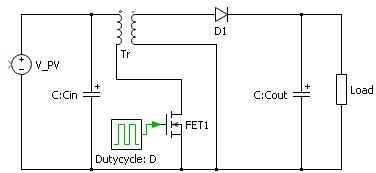
\includegraphics[width=0.7\textwidth]{../Pictures/flyback_schem.png}
	\caption{Flyback converter}
	\label{Flyback_SCHEMATIC}
	\end{center}
\end{figure}

When the MOSFET is on, the energy is transferred from the input voltage source to the transformer. In this state the output capacitor will supply the load with the output voltage. In the off-state the transformer will supply the output load with energy while it charges the capacitor as well.

"Wiki" 

Because of the single control device another advantage of the flyback converter is a wide choice of controllers. For example it is possible to directly connect a PWM controlled IC to control the MOSFET, and by that the converter. 

The drawbacks are primary the current and voltage waveforms. The stress on the switch and diode can be high and comes as a function of the turns ratio of the transformer. Furthermore the leakage inductance from the transformer will result in a big voltage spike at the rising edge of the MOSFET. This needs to be reduced by a snubber circuit. This will increase the power loss and efficiency though. The leakage inductance will also produce transients which will make the voltage stress at the FET bigger and give high-frequency ringing at the input. Lastly there will be increased noise at both terminals due to the fact that the input and output currents are discontinous. 

"Non inverting buckboost texasConverter"



\section{Non-inverting buck-boost converter\label{N_INV_BB}}
		
The Non-inverting Buck-Boost converter is a DC to DC converter that allows the voltage at its output to be higher or lower than the voltage at its input. The topology can be seen in figure \ref{N_INV_BB_SCHEMATIC}. It uses 4 switches, of which 2 are controlled devices. 
		

\begin{figure}[htbp]
	\begin{center}
	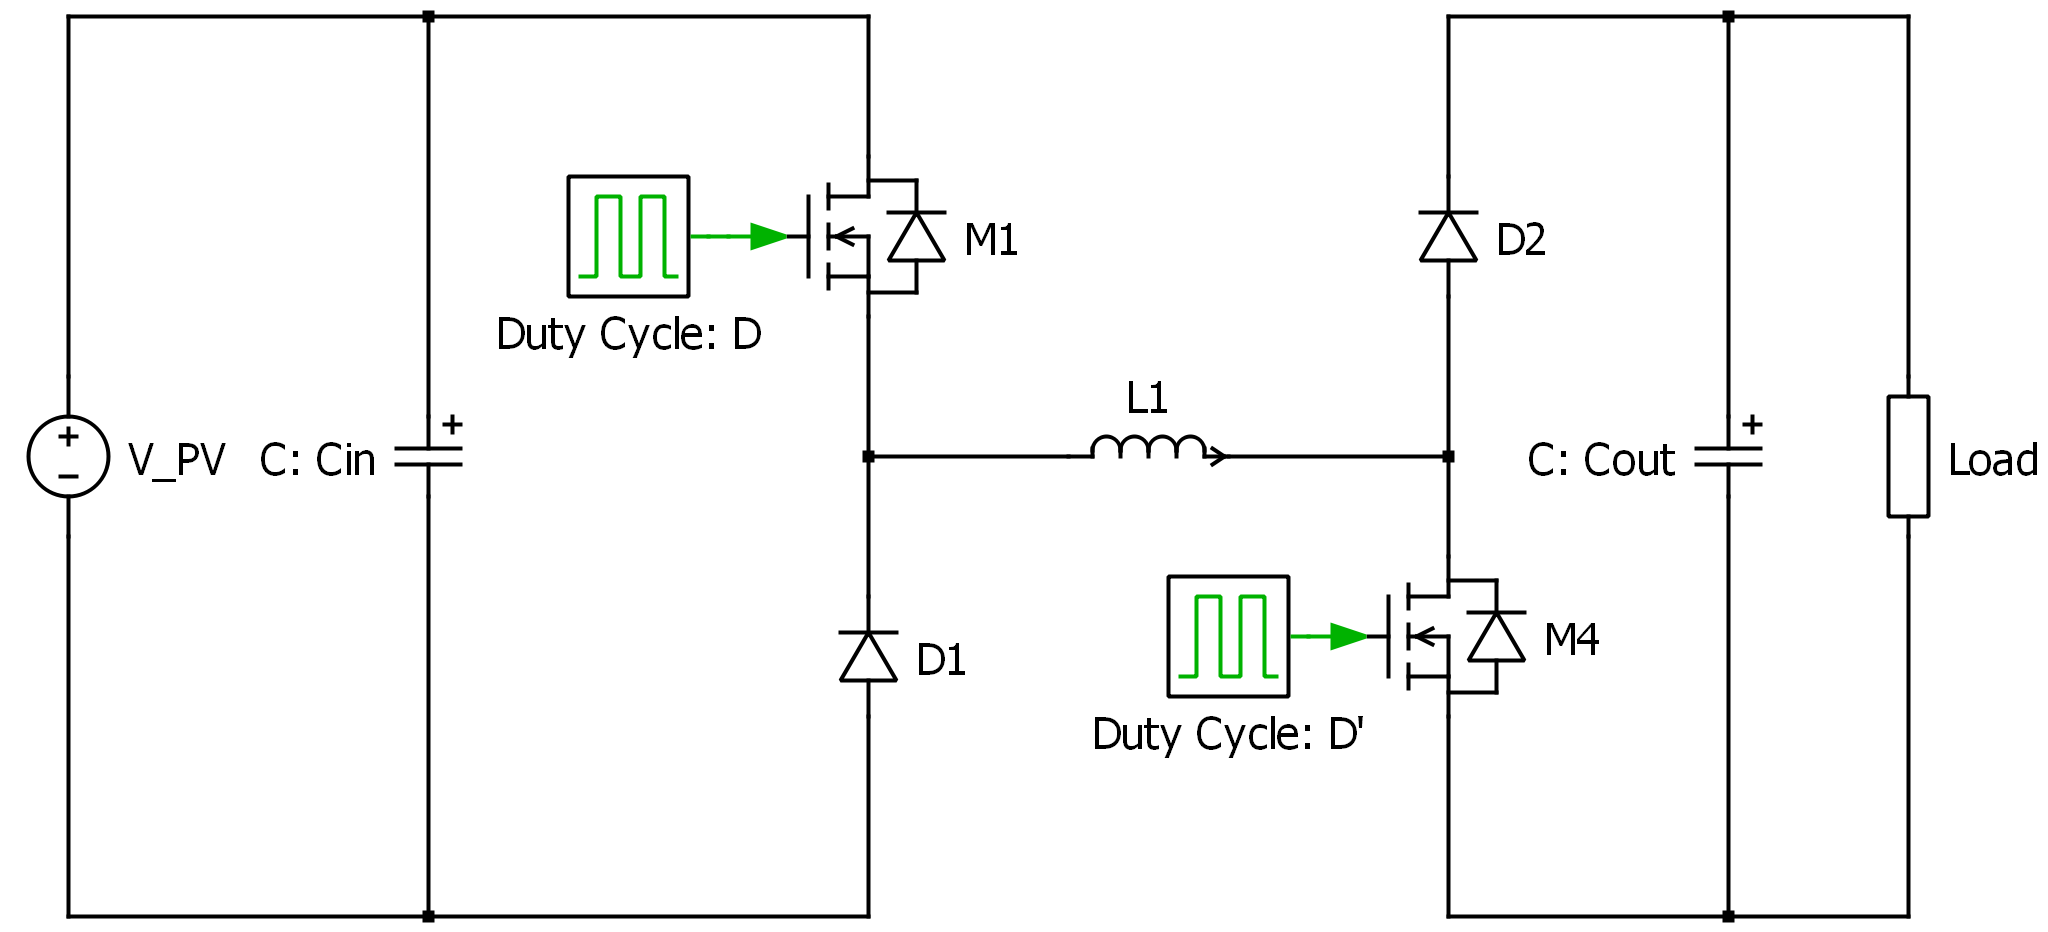
\includegraphics[width=0.7\textwidth]{../Pictures/2_d_H_B_BB}
	\caption{Non-inverting buck-boost converter.}
	\label{N_INV_BB_SCHEMATIC}
	\end{center}	
\end{figure}

		
The controller can force the system to work in any of the following modes:

\begin{enumerate}
	\item Buck $\rightarrow$ $ D \subset [0,1];	 D' = 0 $
	\item Boost $\rightarrow$ $ D = 1;	 D' \subset [0,1] $
	\item Buck-Boost $\rightarrow$ $ D \subset [0,1]; D' \subset [0,1] $
\end{enumerate}
		
Usually the inverter's input voltage is fixed to some value higher than the grid's voltage. The possibility of higher and lower voltages at the converter's output allows different ways of associating photovoltaic modules. Then the user is able to arbitrarily decide how many PV modules to link in series. Differently of what would happen in the case of Buck or Boost converters where the constraints regarding the number of panels are tighter.
		
Compared with other topologies that can have both higher and lower voltages at the output, such as the SEPIC converter, this DC-DC features a single inductor and no intermediate capacitor. See SEPIC schematic in figure \ref{SEPIC_SCHEMATIC}, notice the additional inductor and capacitor. With such reduction in passive components the price, efficiency and power density improves significantly \cite{underthehood}.

\begin{figure}[htbp]
	\begin{center}
		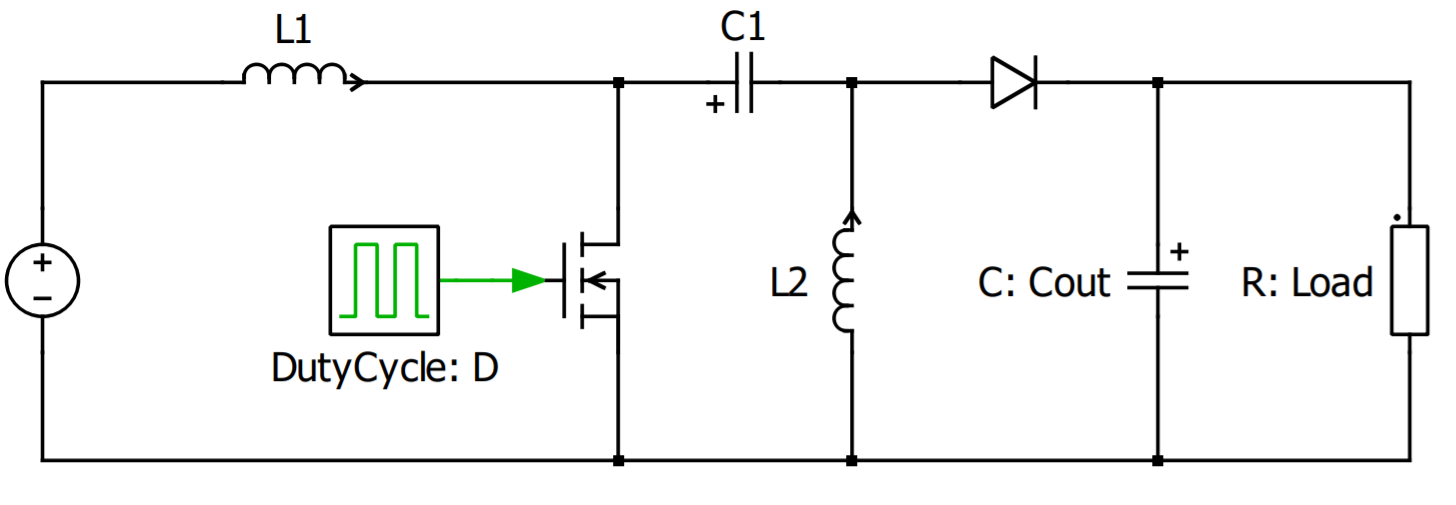
\includegraphics[width=0.7\textwidth]{../Pictures/SEPIC}
		\caption{SEPIC converter.}
		\label{SEPIC_SCHEMATIC}
	\end{center}	
\end{figure}

One of the main drawbacks of the topology is the control's complexity, which must calculate the appropriate duty cycle $D$ and $D'$ in any of the modes and also the transition between these modes. The Buck-Boost mode is specially complicated as there are two duty cycles to calculate. This problem might be addressed by setting a constant duty cycle in one of the bridge's legs and then the control will calculate the other leg's duty cycle  \cite{AN4449_ST}.
		
Although this topology exhibits appropriate features, it can be further improved by replacing the diodes by MOSFETs. The circuit may be seen in figure \ref{BID_N_INV_BB_SCHEMATIC}, it's called Bidirectional Non-Inverting Buck-Boost converter. With this variation, the following changes occur:
		
\begin{enumerate}
	\item The system becomes bidirectional.
	\item The conduction losses are smaller. 
\end{enumerate}
	
If the system is bidirectional it can be used in different MIC strategies, as the topology seen in figure \ref{BID_MIC_ARCHITECTURES}, which features an isolated dc link. This topology needs a bidirectional MIC as energy flow in both directions is needed. It also allows diagnosis of PV modules, as described in section \ref{selection_of_topology}.

\begin{figure}[htbp]
	\begin{center}
		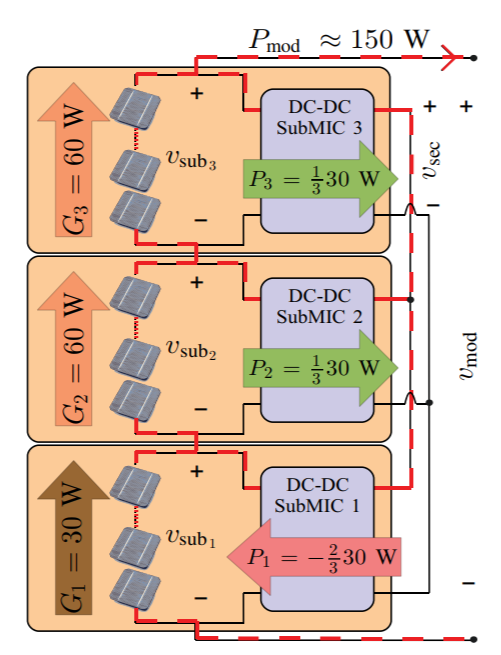
\includegraphics[width=0.4\textwidth]{../Pictures/bidirectional_mic_use}
		\caption{Bidirectional MIC use\cite{ArchitectureMIC}.}
		\label{BID_MIC_ARCHITECTURES}
	\end{center}	
\end{figure}
		
		
As seen in figure \ref{BID_N_INV_BB_SCHEMATIC}, notice that duty cycles of the switches that replace the diodes are $\overline{D}$ and $\overline{D'}$. This line over the variables means that it is the negated value of the original variable. The duty cycle is the boolean variable that indicates the conduction state of a switch. In the case of an enhancement switch, the switch is conducting whenever its driving duty cycle is equal to '1' and it is closed when its driving duty cycle is equal to '0'. 
		
The main drawback is the increased difficulty of the driver circuitry. And the requirement of a dead time in order to avoid the short circuit of $FET_1$ and $FET_3$ or $FET_2$ and $FET_4$ which could damage the system. When using diodes, the system is intrinsically protected against a shoot-through event. 	
		
\begin{figure}[htbp]
	\begin{center}
	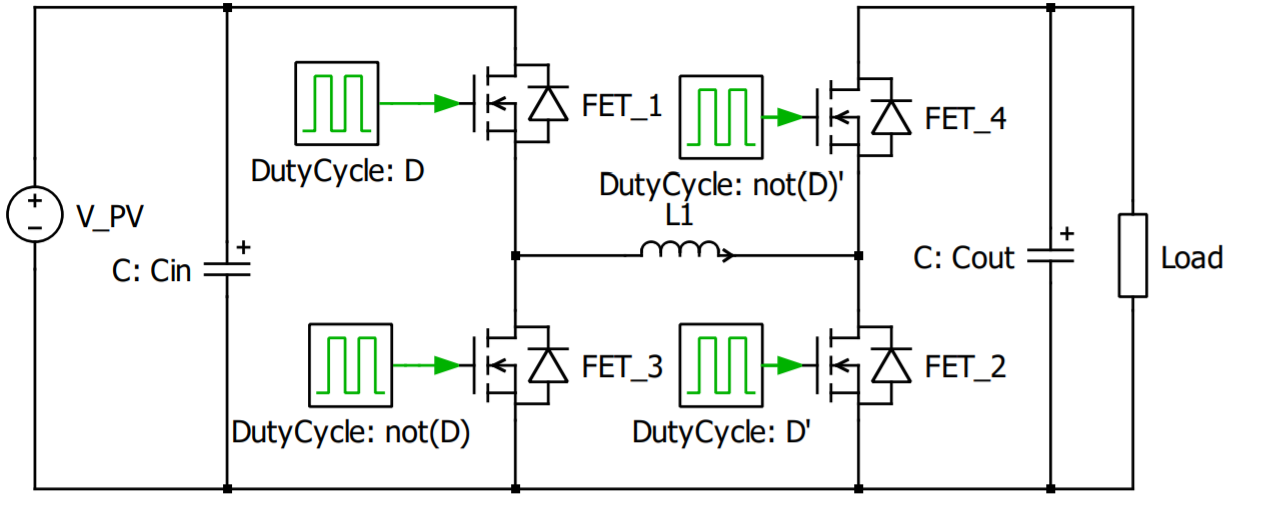
\includegraphics[width=0.7\textwidth]{../Pictures/BID_H_B_BB}
	\caption{Bidirectional Non-inverting buck-boost converter.}
	\label{BID_N_INV_BB_SCHEMATIC}
	\end{center}
\end{figure}





\section{Selection of topology}
The selection of converter topology will be made from the research made earlier in this chapter. The converter should be able to allow both a higher and a lower output than the input. This requirement will limit the buck and boost converters, which converts either up or down. This means that before the requirement is met, both a buck and boost converter must be a part of the implementation. This is not desirable, because it will introduce unnecessary work.  

The next requirement states that the converter should have as high an efficiency as possible. The flyback converter will have a lower efficiency than the buck-boost, because of the transformer. This will introduce a loss in the extra inductor winding, and a larger loss in the FET because of the turns ratio in the transformer. Using a 4 transistor buck-boost converter, instead of a 2 transistor, it is possible to further optimizing the power loss because of the use of FET's instead of diodes. 

The 4 transistor buck-boost converter does also have the advantage of being bidirectional. This means that it's possible to either extract current from the PV-module to the inverter at the output, or to inject current from the inverter to the PV-module. Due to that the PV-modules acts like LEDs, they will radiate an infrared light if current are injected. If the PV-modules are damaged in some way, i.e. having cracks, the radiation will be affected. This means that it is possible to discover faulty modules before efficiency drops. This will increase the overall efficiency of the system and ease the maintenance sequence significantly. 

The Bidirectional Non-Inverting Buck-Boost converter is chosen because of these arguments. However the bidirectional functionality will not be addressed in this project, but could be a part of further development of the converter. 






 
\chapter{Problem Analysis}

\section{Specifications}

\section{Research Question}
\chapter{Existing solutions for Module Integrated Converter}\label{background}

The main topic for this project consist on designing a MIC which basically is a DC-DC converter and a MPPT controller. Therefore, this chapter first analyzes different topologies for DC-DC converter commonly used in MICs. This chapter also gives some background information of the most common MPPT techniques.



\section{Topologies of DC-DC converters}\label{DC_DC_Converters}

\subsection{Buck converter\label{Buck-C}}

A buck converter is one of the simplest DC-DC converters with the task of decreasing the input voltage. The required components are a DC-source for the input voltage, two switches (a diode and a transistor), an inductor, a capacitor and a load. The equivalent diagram in figure \ref{Buck-converter} illustrates a buck-converter \todo{why buck-converter separated like that? Stef}. 

\begin{figure}[htbp]
	\begin{center}
		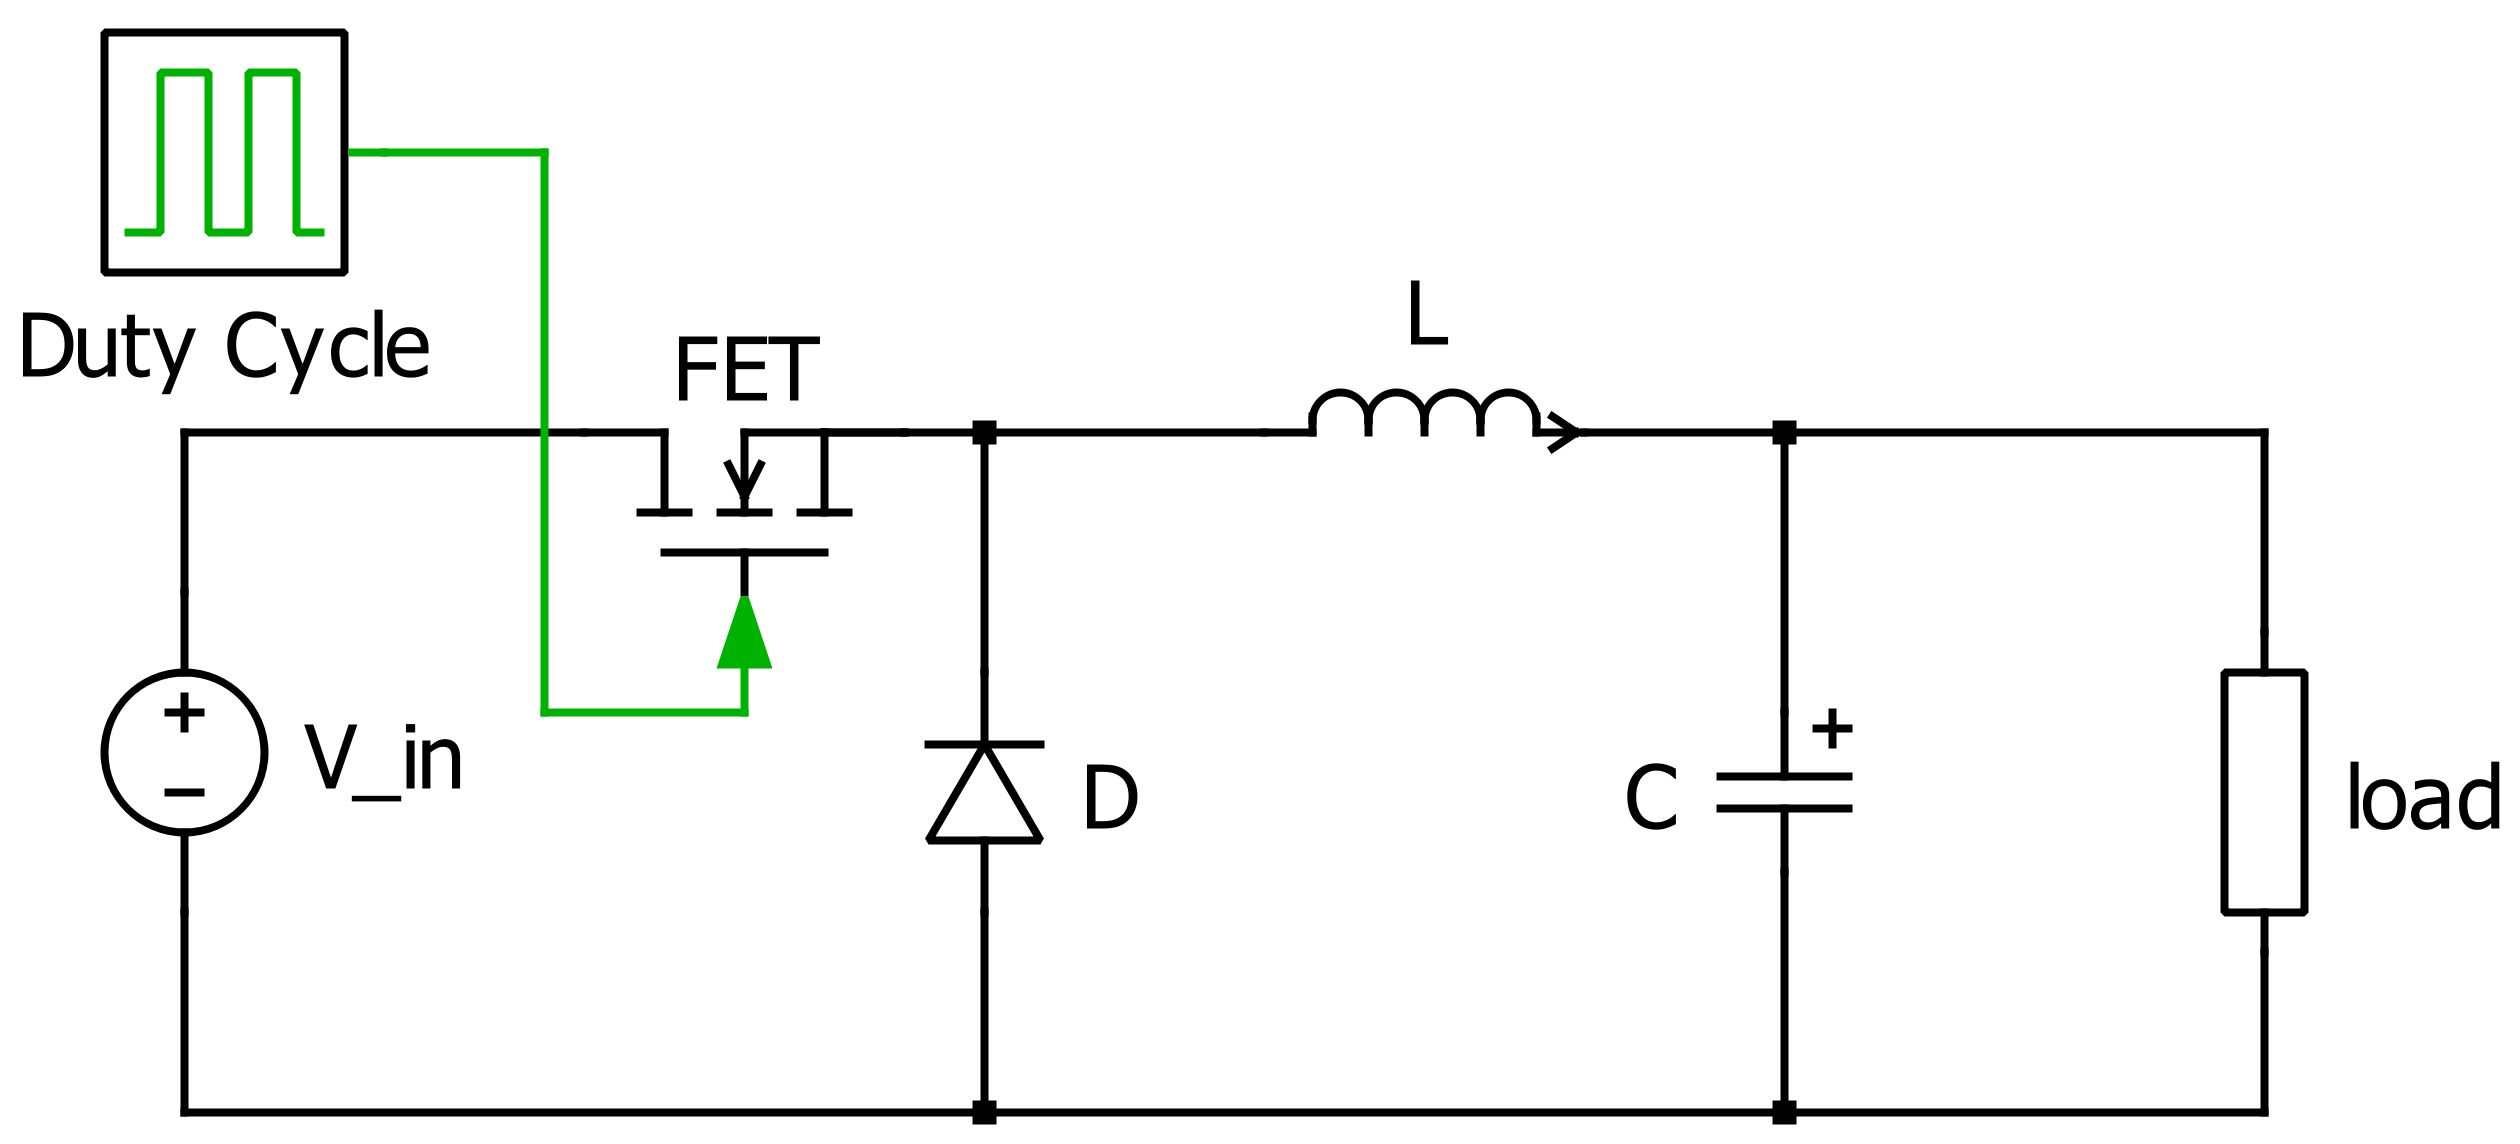
\includegraphics[width=0.7\textwidth]{../Pictures/Buck-converter}
		\caption{Equivalent circuit for the DC-DC buck converter.}
		\label{Buck-converter}
	\end{center}	
\end{figure}
\todo{I've changed the figure's name. Stef}

A buck-converter performs in two operating states. 
During the first state, the MOSFET is conducting and the diode is working as an open-circuit, the voltage drop  then is divided between the inductor and load. Since the voltage is split, the voltage drop on the load is lower than the one of the input source. In addition, both the capacitor and the inductor are being charged. In the second state, the MOSFET is switched off and the current flows through the diode. During this state, the inductor works as a current source and the capacitor stabilizes the voltage \cite{schematicbuckandboost}.

The main advantage for using the buck converter is that the structure is very simple and only one controlled  switch is needed. Also, the component count and thus cost of components is low. Furthermore, the buck converter can reach efficiencies up to 99\% \cite{Efficiencybuck}. 

However, this topology is not very versatile since it does not allow the increase of output voltage with respect to the input. Another drawback is the lack of galvanic isolation between the input and the output \cite{advantagebuck}.
%%http://www.completepowerelectronics.com/buck-converter-tutorial-topology-working-advantages-applications/

\subsection{Boost converter\label{Boost-C}}

A boost converter is another type of DC-DC converter, it is similar to the buck but instead of lowering the output voltage, it produces a higher electrical potential at the output with respect to that at the input.

The circuit consists of two switches (a transistor and a diode), an inductor, a capacitor, a load and a DC-source for the input voltage. Figure \ref{Boost-converter} shows an equivalent circuit diagram with the aforementioned components. %%\cite{Reddy2011}

\begin{figure}[htbp]
	\begin{center}
		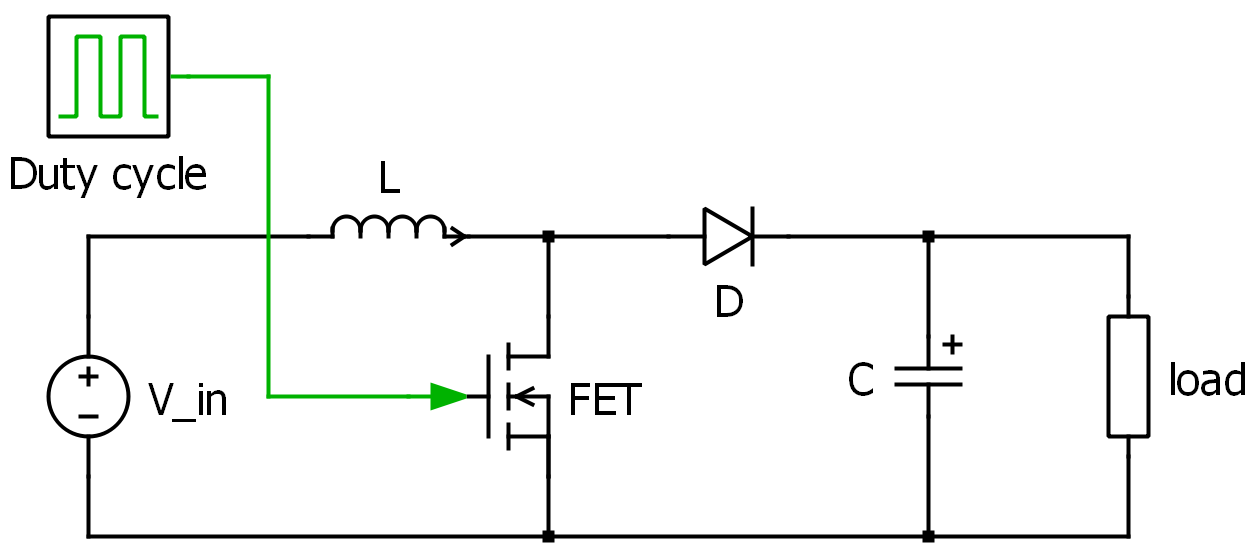
\includegraphics[width=0.7\textwidth]{../Pictures/Boost-converter}
		\caption{Equivalent circuit for the DC-DC boost converter.}
		\label{Boost-converter}
	\end{center}	
\end{figure}

Similarly to the buck converter, this topology has two states, when the MOSFET is on, the current flows only trough the inductor because the diode  is working as an open-circuit. Energy is then stored in the inductor, which voltage is equal to the input voltage, and current increases. Meanwhile, the capacitor releases the previously stored energy to the load.
During the second state, the MOSFET is turned off, the current then loops trough the inductor, diode, capacitor and the load. Since the inductor had been previously charged, it now works as a current source in series with the voltage source of the circuit. The voltage across the load is then risen with respect to that at the input. Furthermore, the capacitor is charging \cite{schematicbuckandboost}.

An advantage for a boost converter is that it can raise the output voltage without using a transformer. It is also a cheap converter easy to control \cite{advantageboost}. 

However, as it happened with the buck, the boost converter is also limited to rising the voltage and lowering it cannot be achieved. Also, if an error happens in the control of the MOSFET and it is left in ON-mode for a long time, a short-circuit is created and the current will increase until a component fails. Finally, this converter does not have galvanic isolation either. 
 



\section{Non-inverting buck-boost converter\label{N_INV_BB}}
		
The Non-inverting Buck-Boost converter is a DC to DC converter that allows the voltage at its output to be higher or lower than the voltage at its input. The topology can be seen in figure \ref{N_INV_BB_SCHEMATIC}. It uses 4 switches, of which 2 are controlled devices. 
		

\begin{figure}[htbp]
	\begin{center}
	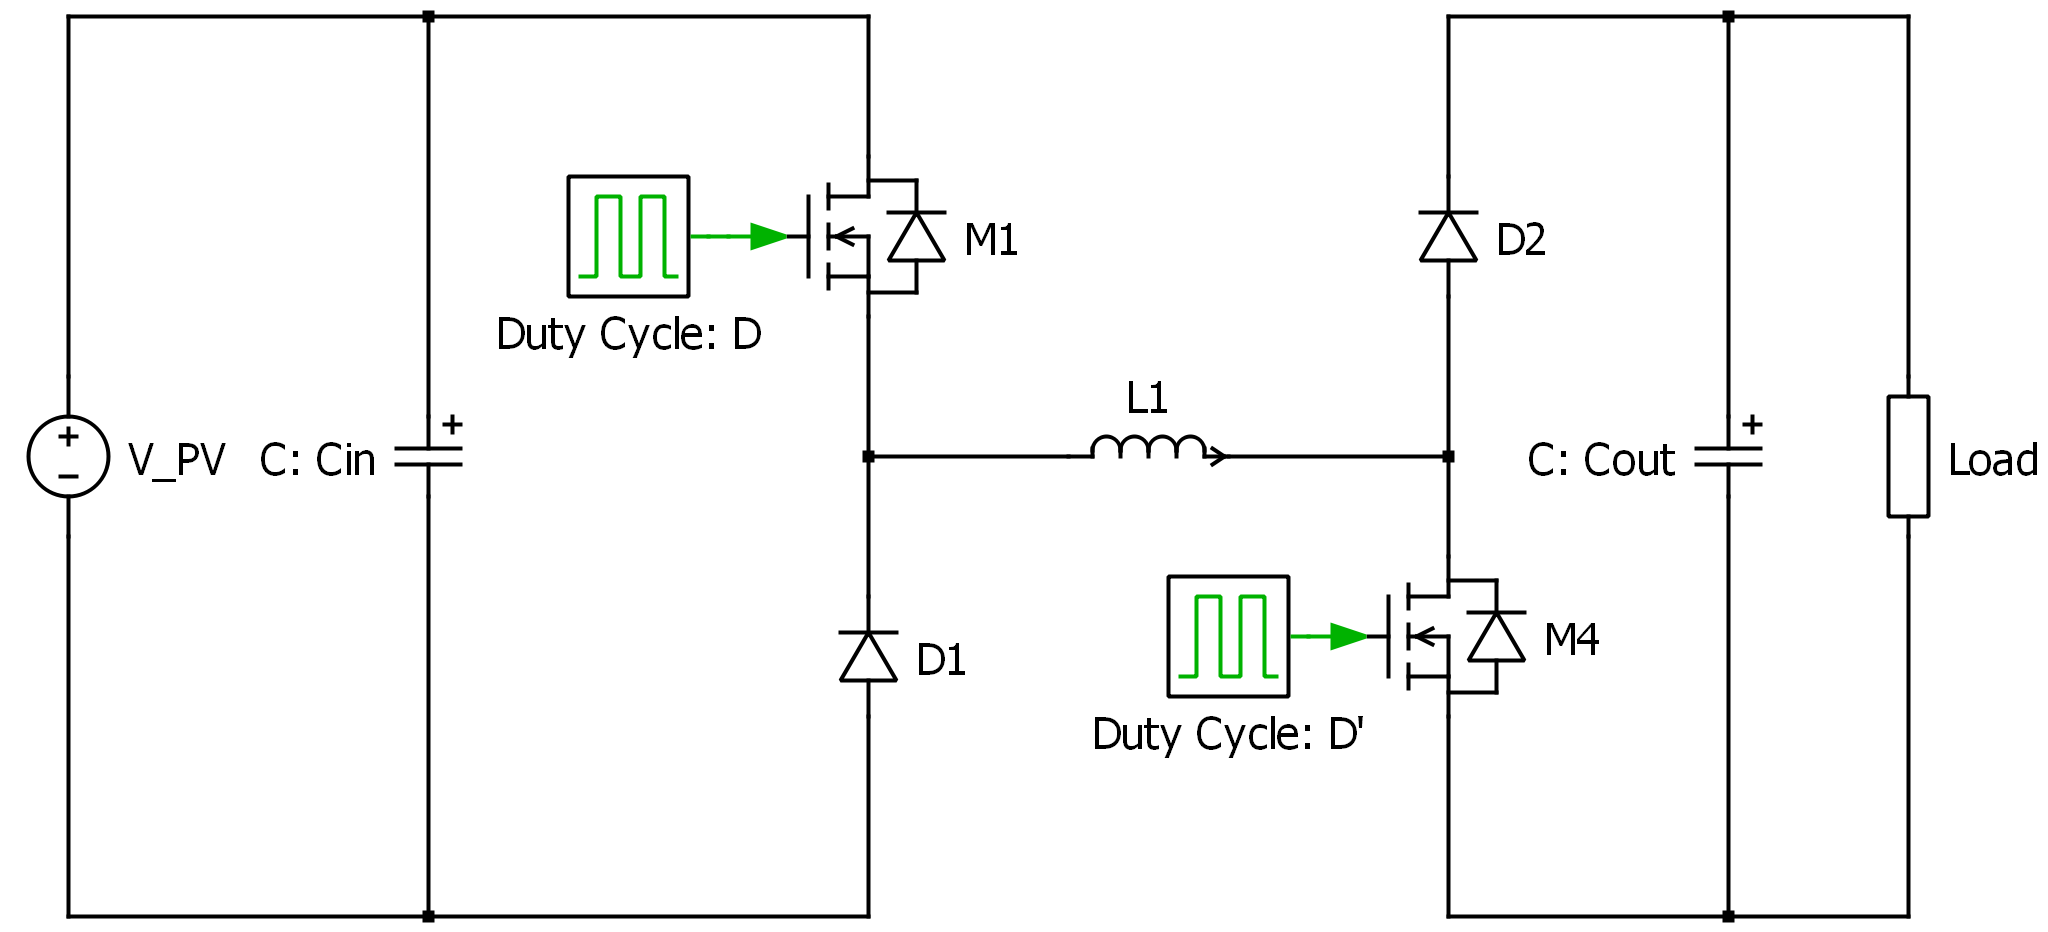
\includegraphics[width=0.7\textwidth]{../Pictures/2_d_H_B_BB}
	\caption{Non-inverting buck-boost converter.}
	\label{N_INV_BB_SCHEMATIC}
	\end{center}	
\end{figure}

		
The controller can force the system to work in any of the following modes:

\begin{enumerate}
	\item Buck $\rightarrow$ $ D \subset [0,1];	 D' = 0 $
	\item Boost $\rightarrow$ $ D = 1;	 D' \subset [0,1] $
	\item Buck-Boost $\rightarrow$ $ D \subset [0,1]; D' \subset [0,1] $
\end{enumerate}
		
Usually the inverter's input voltage is fixed to some value higher than the grid's voltage. The possibility of higher and lower voltages at the converter's output allows different ways of associating photovoltaic modules. Then the user is able to arbitrarily decide how many PV modules to link in series. Differently of what would happen in the case of Buck or Boost converters where the constraints regarding the number of panels are tighter.
		
Compared with other topologies that can have both higher and lower voltages at the output, such as the SEPIC converter, this DC-DC features a single inductor and no intermediate capacitor. See SEPIC schematic in figure \ref{SEPIC_SCHEMATIC}, notice the additional inductor and capacitor. With such reduction in passive components the price, efficiency and power density improves significantly \cite{underthehood}.

\begin{figure}[htbp]
	\begin{center}
		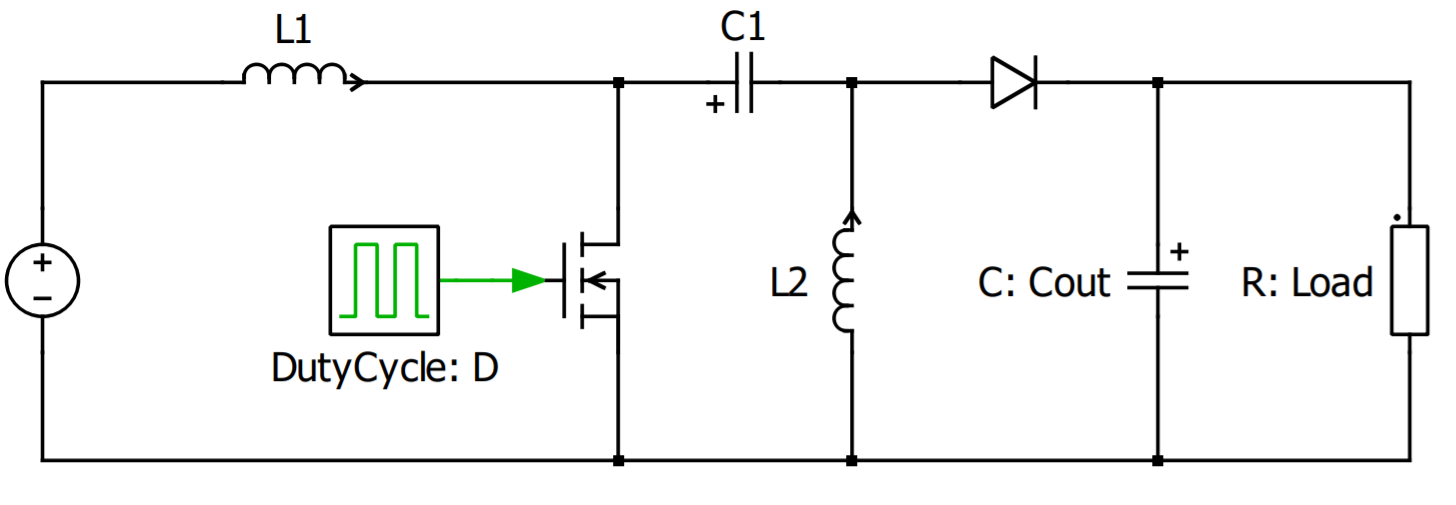
\includegraphics[width=0.7\textwidth]{../Pictures/SEPIC}
		\caption{SEPIC converter.}
		\label{SEPIC_SCHEMATIC}
	\end{center}	
\end{figure}

One of the main drawbacks of the topology is the control's complexity, which must calculate the appropriate duty cycle $D$ and $D'$ in any of the modes and also the transition between these modes. The Buck-Boost mode is specially complicated as there are two duty cycles to calculate. This problem might be addressed by setting a constant duty cycle in one of the bridge's legs and then the control will calculate the other leg's duty cycle  \cite{AN4449_ST}.
		
Although this topology exhibits appropriate features, it can be further improved by replacing the diodes by MOSFETs. The circuit may be seen in figure \ref{BID_N_INV_BB_SCHEMATIC}, it's called Bidirectional Non-Inverting Buck-Boost converter. With this variation, the following changes occur:
		
\begin{enumerate}
	\item The system becomes bidirectional.
	\item The conduction losses are smaller. 
\end{enumerate}
	
If the system is bidirectional it can be used in different MIC strategies, as the topology seen in figure \ref{BID_MIC_ARCHITECTURES}, which features an isolated dc link. This topology needs a bidirectional MIC as energy flow in both directions is needed. It also allows diagnosis of PV modules, as described in section \ref{selection_of_topology}.

\begin{figure}[htbp]
	\begin{center}
		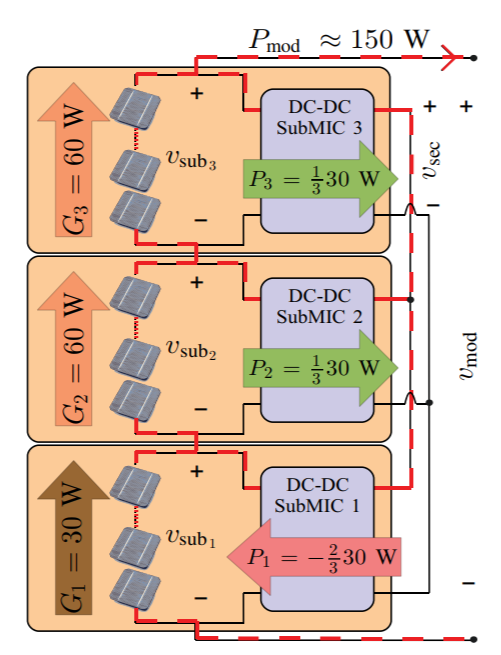
\includegraphics[width=0.4\textwidth]{../Pictures/bidirectional_mic_use}
		\caption{Bidirectional MIC use\cite{ArchitectureMIC}.}
		\label{BID_MIC_ARCHITECTURES}
	\end{center}	
\end{figure}
		
		
As seen in figure \ref{BID_N_INV_BB_SCHEMATIC}, notice that duty cycles of the switches that replace the diodes are $\overline{D}$ and $\overline{D'}$. This line over the variables means that it is the negated value of the original variable. The duty cycle is the boolean variable that indicates the conduction state of a switch. In the case of an enhancement switch, the switch is conducting whenever its driving duty cycle is equal to '1' and it is closed when its driving duty cycle is equal to '0'. 
		
The main drawback is the increased difficulty of the driver circuitry. And the requirement of a dead time in order to avoid the short circuit of $FET_1$ and $FET_3$ or $FET_2$ and $FET_4$ which could damage the system. When using diodes, the system is intrinsically protected against a shoot-through event. 	
		
\begin{figure}[htbp]
	\begin{center}
	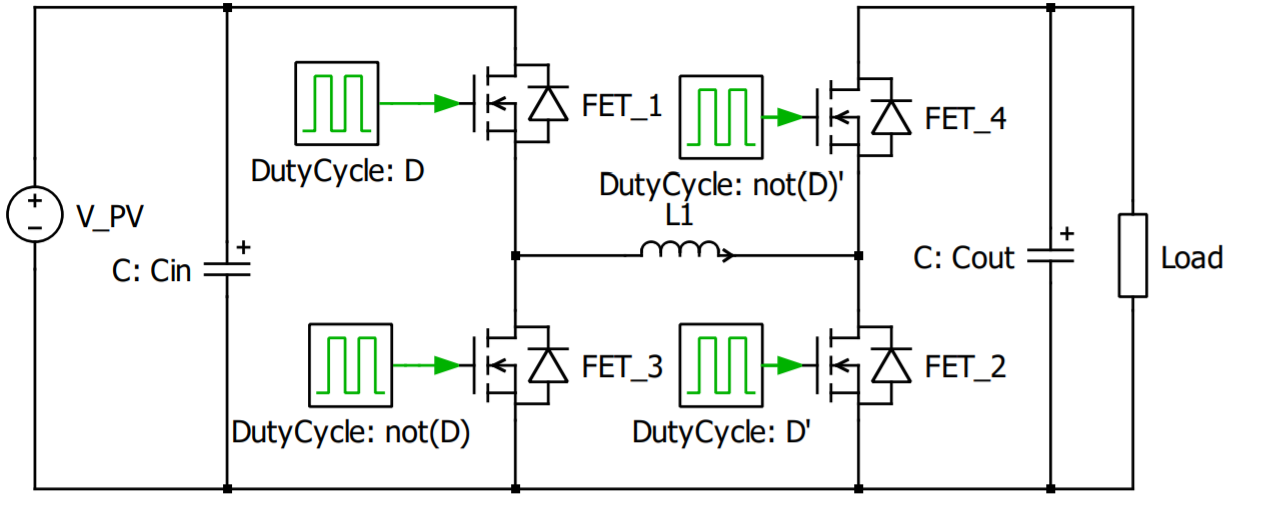
\includegraphics[width=0.7\textwidth]{../Pictures/BID_H_B_BB}
	\caption{Bidirectional Non-inverting buck-boost converter.}
	\label{BID_N_INV_BB_SCHEMATIC}
	\end{center}
\end{figure}





\section{Evaluation of main MPPT techniques\label{MPPTalgo}}

There are a variety of different techniques for finding the maximum power point. Therefore only three different methods are used in this thesis, otherwise it would go beyond the scope of this work. These three methods are the perturb and observe, constant voltage and incremental conductance. Perturb and observe and incremental conductance are the most used algorithms in commercial pv-panels. On the other hand, constant voltage has been selected as a comparison to methods that are not used so often. The reason for that is there other methods which are easier to implement but they have a high disadvantage.\todo{why as a comparison? AT}. 

\subsection{Constant voltage}
Empirical experiments have shown that the voltage of the MPP has a linear dependence on the open circuit voltage at different ambient conditions.

\begin{equation} \label{voltage_MPP}
V_{MPP} = k * V_{OC}	
\end{equation} 
In the equation \ref{voltage_MPP} k represents a constant that depends on the characteristics of the respective pv panel. To determine the value for k, the voltage for MPP and open circuit must be recorded for each temperature and solar irradiation. According to different papers, this value lies between 70 and 80 percent\cite{MPPTresearch}. The algorithm starts with the recording of the open circuit voltage and a predetermined k-value \todo{the k value is not detected... AT}. In each iteration step the $V_{MPP}$ is calculated first. After this, the operating voltage is compared with the calculated voltage of the MPP. If the voltage is not equal, the constant k is changed for the next iteration step to reach the MPP. When the algorithm has reached the MPP, the algorithm is stopped, as you can see in the flowchart in the figure \ref{fcconstantvoltage}\cite{flowchartVC}. \todo{how is the constant k calculated? I thought this method had a constant k determined by the characteristics of the pv, maybe im wrong but we should revise it. AT}

\begin{figure}[htbp]
	\begin{center}
		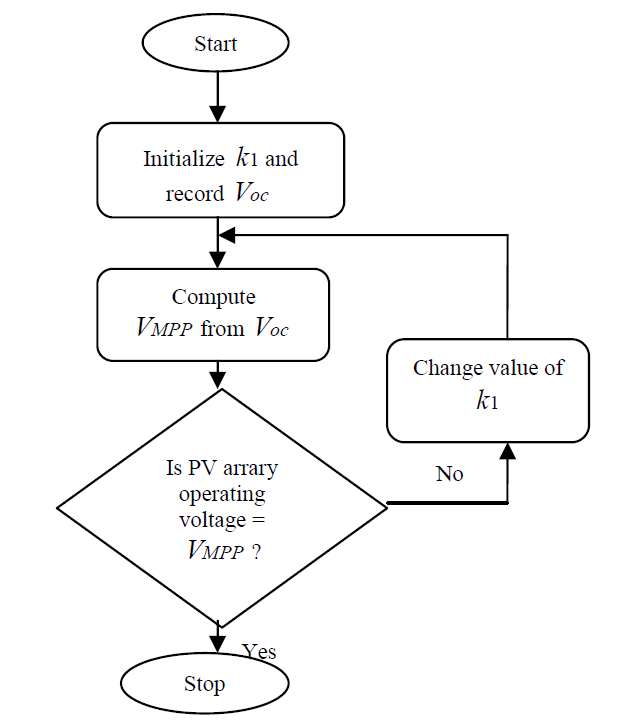
\includegraphics[width=0.5\textwidth]{../Pictures/P1/Flow_chart/Flow_chart_constant_voltage}
		\caption{flow chart constant voltage\cite{flowchartVC}. }
		\label{fcconstantvoltage}
	\end{center}	
\end{figure}

\subsection{Perturb and observe}
With the method "perturb and observe", the currently measured power is periodically compared with the previous power. If the measured power is greater than the power from the previous measurement, the voltage is further increased to reach the MPP. If a power reduction is detected after the comparison, the voltage is reduced \todo{this is not always true... depends on what side of the MPP we are working at. AT}. The flowchart in the figure \ref{fcperturbandobserve} illustrates this method. The classical algorithm uses a fixed step to change the voltage. When the MPP is reached, the algorithm oscillates around the MPP\cite{flowchartVC}. 

\begin{figure}[htbp]
	\begin{center}
		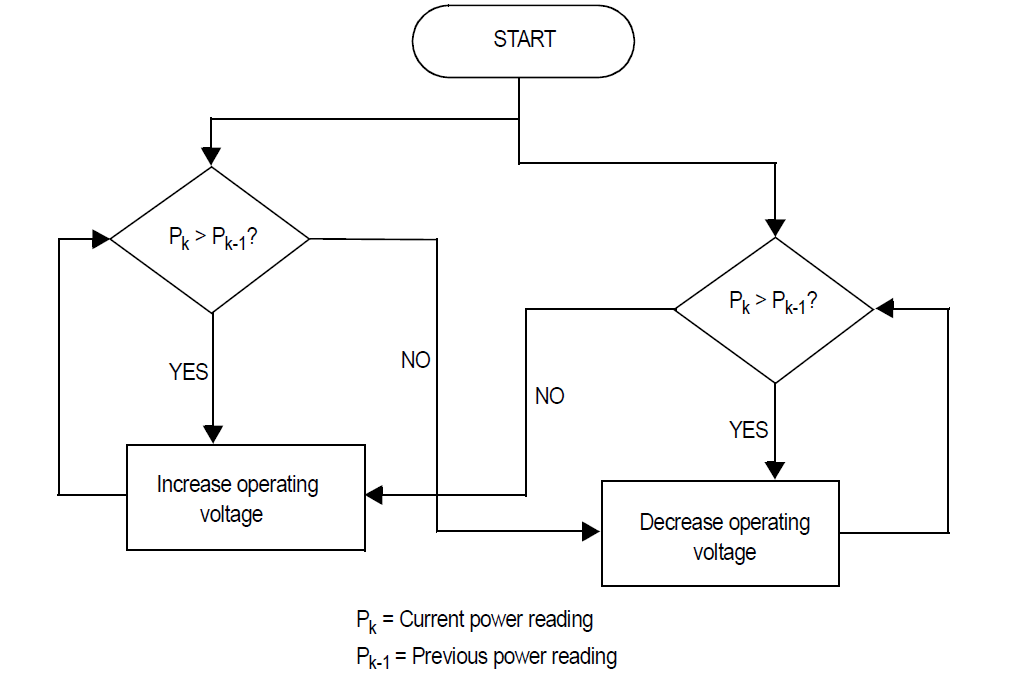
\includegraphics[width=0.7\textwidth]{../Pictures/P1/Flow_chart/flow_chart_perturb_observe}
		\caption{flow chart from perturb and observe\cite{AN1521_MC}.}
		\label{fcperturbandobserve}
	\end{center}	
\end{figure}

\subsection{Incremental conductancee}
The approach of incremental conductance is that the MPP is at the position where the derivative of the power with respect to the voltage is 0. On the left side of the MPP the derivative is greater than 0 while on the right side it is less than 0, this behavior is described by the following equations.\todo{I'll give you the equations later.}\newline
The algorithm compares the incremental conductance with the previous one to increase (left side of MPP) or decrease (right side of MPP) the voltage. After the MPP has been reached, the algorithm is stopped. Thus, there will be no oscillation around the MPP. If a change in the current is detected, the algorithm starts to find the MPP again, as you can see in the flowchart in the figure \ref{fcinccon}\cite{AN1521_MC}.
\begin{figure}[H]
	\begin{center}
		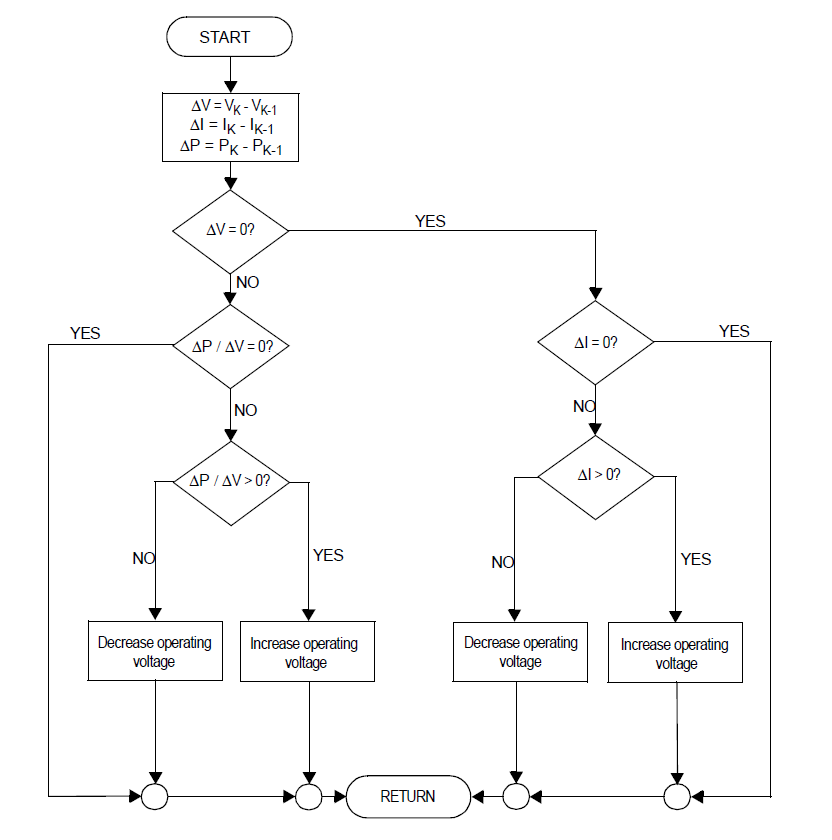
\includegraphics[width=0.7\textwidth]{../Pictures/P1/Flow_chart/flow_chart_incremental_conductance}
		\caption{flow chart incremental conductance \cite{AN1521_MC} }
		\label{fcinccon}
	\end{center}	
\end{figure}
\todo{also a bit small of a figure, the text should be around the same size of the rest of the words i would say. AT}


\section{Future work}
This section will describe the planned future work of the project. This includes parts that were prioritized low or Simplified to achieve a working converter. Furthermore it includes improvements that was discovered during both the development and testing period of the project.

%4- Recommendations for future work. Make general statements. Items: a)what study is needed, b)Methods to be used, c)what is needed for that study.

\subsection{MPPT technique}
Even though the P\&O algorithm was implemented, initial research showed that the incremental conductance method could have been a better option.  Further research and simulations will have to be made for comparing the two methods. \todo{Write about what could be gained from changing MPPT, NHF.}

\subsection{V/I controller}


\subsection{Hardware improvements}
In the first iterations of the converter design, the driver circuits have been designed using isolated power supplies for the high side drivers. These are costly both in size and money wise. Because of that it's preferable to implement a bootstrap circuit for the drivers. An option for a driver including bootstrap could be UCC27211 \cite{boot_driver_datasheet}. This includes both a high and low side driver, such that only to IC's are necessary for the converter. The input threshold is below $2.8V$ for both sides, which means that a $5V$ optocoupler could be used for isolation. For cost and size optimization the optocouplers should be one quad optocoupler, instead of four singles. 
 
%bootstrap, change driver to the A version due to voltage levels and then change the optocouupler to a quad version, control system powered from pv-panel, \dots

\subsection{Coil design}
The coil used for the converter is reused from an earlier project. Measurements shows that it's oversized regarding current ratings. To achieve an optimal coil it should be designed for this specific converter. Both the core size and wire diameter depends on the wanted current rating of the converter \cite{underthehood}. Because of this it will be possible to lower both the cost and size of the coil. 

\subsection{Switching frequency limitations}

%\subsection{Component price, system size, optimization needed}
%Component prize and system size will be introduced during the other sections...

\subsection{Efficiency}
The main purpose of the MIC is to maximize the output efficiency of a PV-panel. To achieve that, the efficiency of the converter itself should be maximized. During the tests, the efficiency was measured to \textit{ADD SOME NICE DATA}\todo{Insert measured efficiency, NHF.}. Other papers shows that an efficiency of up to $95-96\%$ should be achievable\cite{underthehood}, \cite{efficient_buckboost}. 
\chapter{Appendix}

\section{PBL} 

Problem Based Learning $(PBL)$ is a method to organize the group work which will help to approach the projects objectives. Collaboration in the group is a very important factor to get the project working as efficient and fluent as possible.
Therefore there has initially been put some work into a way to work and organize the project. By doing that in the beginning we will save important time later on.
First of all this is a group of 6 people so it is important to give different tasks to different people to keep it efficient. 

To make sure everyone know what is going on there will be a group meeting at least once a week. Usually there will be more. Here the group members presents their progress for each other and if there has been any problems, it will be discussed here. In these meetings there are one chair-person who needs to make sure that all the topics of the agenda is being discussed. Besides the chair-person there is a referent who writes the minutes-of-meeting. 

A supervisor meeting will be held at least once every two weeks. Again with a chair-person and a referent. Before the meeting the agenda and questions has been sent to the supervisors and afterwards the group will sent the minutes-of-meeting. The goal here is to show the supervisors that the project is moving in the right direction and to get the questions answered. Furthermore the group sends the documentation to get feedback regularly.

To organize the tasks between the group members the web-page Trello is used as a taskboard. All the tasks that should be done is written here and divided the sections "To do", "Doing", "Done". This makes sure that everybody can see which tasks is in progress and who are working on them. A time-plan has been develop using a Gantt chart (Figure \ref{gantt}), so there is a common agreement on which tasks should be done at first.              


%\clearpage

\printbibliography

\end{document}